\begin{frame}
    \frametitle{供給}
    \begin{equation*}
        \ln(QPROD_t) = \beta_1 + \beta_2 \ln(P_t) + \beta_3 \ln(PF_t) + \beta_4 TIME_t + \beta_5 \ln(QPROD_{t-1}) + e_t^s
    \end{equation*}

    內生變數:供給量、價格\\
    外生變數:
    \begin{itemize}
        \item 飼料價格
        \item 年份指數
        \item 上一期的供給量
    \end{itemize}
\end{frame}

\begin{frame}
    \frametitle{單純地進行估計}
    \begin{columns}
        \begin{column}{0.5\textwidth}
            跟前面一樣,先看看常見的錯誤:單純把結構式進行OLS\\[3em]
            
           供給線斜率不顯著為正
        \end{column}

        \begin{column}{0.5\textwidth}
            \begin{table}
                \centering
                \scalebox{0.9}{
                {
\def\sym#1{\ifmmode^{#1}\else\(^{#1}\)\fi}
\begin{tabular}{l*{1}{c}}
\hline\hline
            &\multicolumn{1}{c}{ln\_qprod}\\
\hline
ln\_p        &      0.0252         \\
            &    (0.0671)         \\
[1em]
ln\_pf       &     -0.0999\sym{*}  \\
            &    (0.0421)         \\
[1em]
time        &      0.0113\sym{*}  \\
            &   (0.00503)         \\
[1em]
L.ln\_qprod  &       0.727\sym{***}\\
            &     (0.104)         \\
[1em]
\_cons      &       2.154\sym{**} \\
            &     (0.782)         \\
\hline\hline
\end{tabular}
}

                }
            \end{table}
        \end{column}
    \end{columns}
    

\end{frame}

\begin{frame}[fragile]
    \frametitle{第一階段的顯著性}
    
    \begin{columns}
        \begin{column}{0.5\textwidth}
            工具變數:
            \begin{itemize}
                \item 人均收入
                \item 牛肉價格
                \item 人口成長率
                \item 上一期的出口
            \end{itemize}

            第一階段聯合檢定
            \begin{lstlisting}
test ln_y ln_pb popgro L.lexpts \end{lstlisting}
        \end{column}

        \begin{column}{0.5\textwidth}
            \begin{table}
                \centering
                \scalebox{0.6}{
                {
\def\sym#1{\ifmmode^{#1}\else\(^{#1}\)\fi}
\begin{tabular}{l*{1}{c}}
\hline\hline
            &\multicolumn{1}{c}{ln\_p}\\
\hline
ln\_y        &       0.856         \\
            &     (0.630)         \\
[1em]
ln\_pb       &       0.219         \\
            &     (0.234)         \\
[1em]
popgro      &     -0.0231         \\
            &     (0.118)         \\
[1em]
L.lexpts    &       2.322\sym{**} \\
            &     (0.709)         \\
[1em]
ln\_pf       &       0.177         \\
            &     (0.108)         \\
[1em]
time        &     -0.0505\sym{*}  \\
            &    (0.0216)         \\
[1em]
L.ln\_qprod  &      -0.141         \\
            &     (0.327)         \\
[1em]
\_cons      &      -5.412         \\
            &     (6.297)         \\
\hline\hline
\end{tabular}
}

                }
            \end{table}
        \end{column}
    \end{columns}
\end{frame}

\begin{frame}[fragile]
    \frametitle{作法二}
    也可以直接在 \texttt{ivregress} 
    \begin{lstlisting}
eststo est_2SLS : ivregress 2sls ln_qprod (ln_p = ln_y ln_pb popgro L.lexpts) /// 
    ln_pf time L.ln_qprod, first

estat first\end{lstlisting}
    
    \begin{figure}
        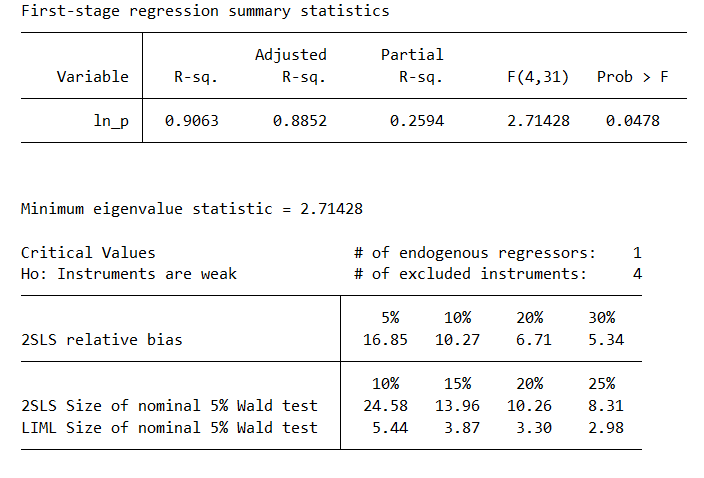
\includegraphics[width=0.8\textwidth]{fig/result_11-12-c.png}
    \end{figure}
\end{frame}

\begin{frame}[fragile]
    \frametitle{供給函數的 2SLS}
\begin{lstlisting}
eststo est_2SLS : ivregress 2sls ln_qprod ///
    (ln_p = ln_y ln_pb popgro L.lexpts) /// 
    ln_pf time L.ln_qprod, first \end{lstlisting}
\end{frame}

\begin{frame}
    \frametitle{結果}

    \begin{table}
        \scalebox{0.9}{
        {
\def\sym#1{\ifmmode^{#1}\else\(^{#1}\)\fi}
\begin{tabular}{l*{3}{c}}
\hline\hline
            &\multicolumn{1}{c}{est\_b}&\multicolumn{1}{c}{est\_2SLS}&\multicolumn{1}{c}{est\_2SLS\_HAC}\\
\hline
ln\_p        &      0.0252         &      0.0446         &      0.0446         \\
            &    (0.0671)         &     (0.123)         &    (0.0891)         \\
[1em]
ln\_pf       &     -0.0999\sym{*}  &      -0.105\sym{*}  &      -0.105         \\
            &    (0.0421)         &    (0.0486)         &    (0.0571)         \\
[1em]
time        &      0.0113\sym{*}  &      0.0120\sym{*}  &      0.0120\sym{*}  \\
            &   (0.00503)         &   (0.00589)         &   (0.00599)         \\
[1em]
L.ln\_qprod  &       0.727\sym{***}&       0.718\sym{***}&       0.718\sym{***}\\
            &     (0.104)         &     (0.110)         &     (0.132)         \\
[1em]
\_cons      &       2.154\sym{**} &       2.214\sym{**} &       2.214\sym{*}  \\
            &     (0.782)         &     (0.800)         &     (1.001)         \\
\hline\hline
\multicolumn{4}{l}{\footnotesize Standard errors in parentheses}\\
\multicolumn{4}{l}{\footnotesize \sym{*} \(p<0.05\), \sym{**} \(p<0.01\), \sym{***} \(p<0.001\)}\\
\end{tabular}
}

        }
    \end{table}
\end{frame}
